\section{Mengdelære}
\subsection{Mengder}
\begin{frame}{Sett / Mengder}
    Et sett, eller en mengde, er en slags liste av objekter, men med to forskjeller:\\
    \indent \hspace{3mm}    1. Det inneholder ingen duplikater\\
    \indent \hspace{3mm}    2. Det har ingen konkret rekkefølge
    
    \pause
    \begin{block}{Eksempel}
        Alle de følgende settene er like: \\
        $\{1, 2, 3\}$, $\{3, 2, 1\}$ \\
        $\{1, 1, 1, 1, 2, 2, 3, 3\}$
    \end{block}
    
    \pause
    \begin{block}{Eksempel}
        $1 \in \{1, 2, 3\}$ = T \\
        $5 \in \{1, 2, 3\}$ = F
    \end{block}
\end{frame}


\begin{frame}{Kjente sett}
    Flere sett bruker vi veldig ofte. Her er noen av dem.\\
    
    \begin{tabular}{c|l|c}
        Symbol & Navn & Innhold \\ \hline
        $\mathbb{N}$ & Naturlige tall & $\{0, 1, 2, 3, ....\}$\\
        $\mathbb{Z}$ & Heltall & $\{... -2, -1, 0, 1, 2, 3, ....\}$\\
        $\mathbb{Q}$ & Rasjonale tall & $\{-3/2, 1/10, 4/5, 5/4, ....\}$\\
        $\mathbb{R}$ & Reelle tall & $\{\pi, e, 0.111111111..., 2\pi, .....\}$\\
        $\emptyset$ & Det tomme settet & $\{\}$
    \end{tabular}
    
\end{frame}

\begin{frame}[fragile]{Settbyggingsnotasjon}
    Istedet for å manuelt skrive opp alle elementene i et sett, eller å bruke uformell \enquote{...}-notasjon, kan vi bruke setbyggingsnotasjon.
    \begin{block}{Eksempler}
        $\{ x | x \in \mathbb{N}\}$ = $\mathbb{N}$\\
        $\{ x \cdot 2 | x \in \mathbb{N}\}$ = $\{0, 2, 4, 6, 8, ....\}$\\
        $\{x | x \in \mathbb{N}, x$ mod $3 = 0 \} = \{0, 3, 6, 9, ...\}$\\
        $\{x/2 | x \in \mathbb{N}, x$ mod $3 = 0\} = \{0, 1.5, 3, 4.5, ...\}$
    \end{block}
    \pause
    \begin{minted}[fontsize=\scriptsize]{python}
\[ x for x in range(100) \]
\[ x*2 for x in range(100) \]
\[ x for x in range(100) if x % 3 == 0 \]
\[ x/2 for x in range(100) if x % 3 == 0 \]
    \end{minted}
\end{frame} 

\begin{frame}{$\cup$, $\cap$, $\bar{}$ og $-$}
    $A \cup B := \{x | x \in A \lor x \in B\}$ \\
    $A \cap B := \{x | x \in A \land x \in B\}$\\
    $A - B = A \backslash B := \{x | x \in A\land  x \notin B\}$\\
    $A^C = \bar{A} := \{x | x \notin A\}$
    
    \pause
    \begin{figure}%
        \centering
        \subfloat[\centering $A \cup B$]{{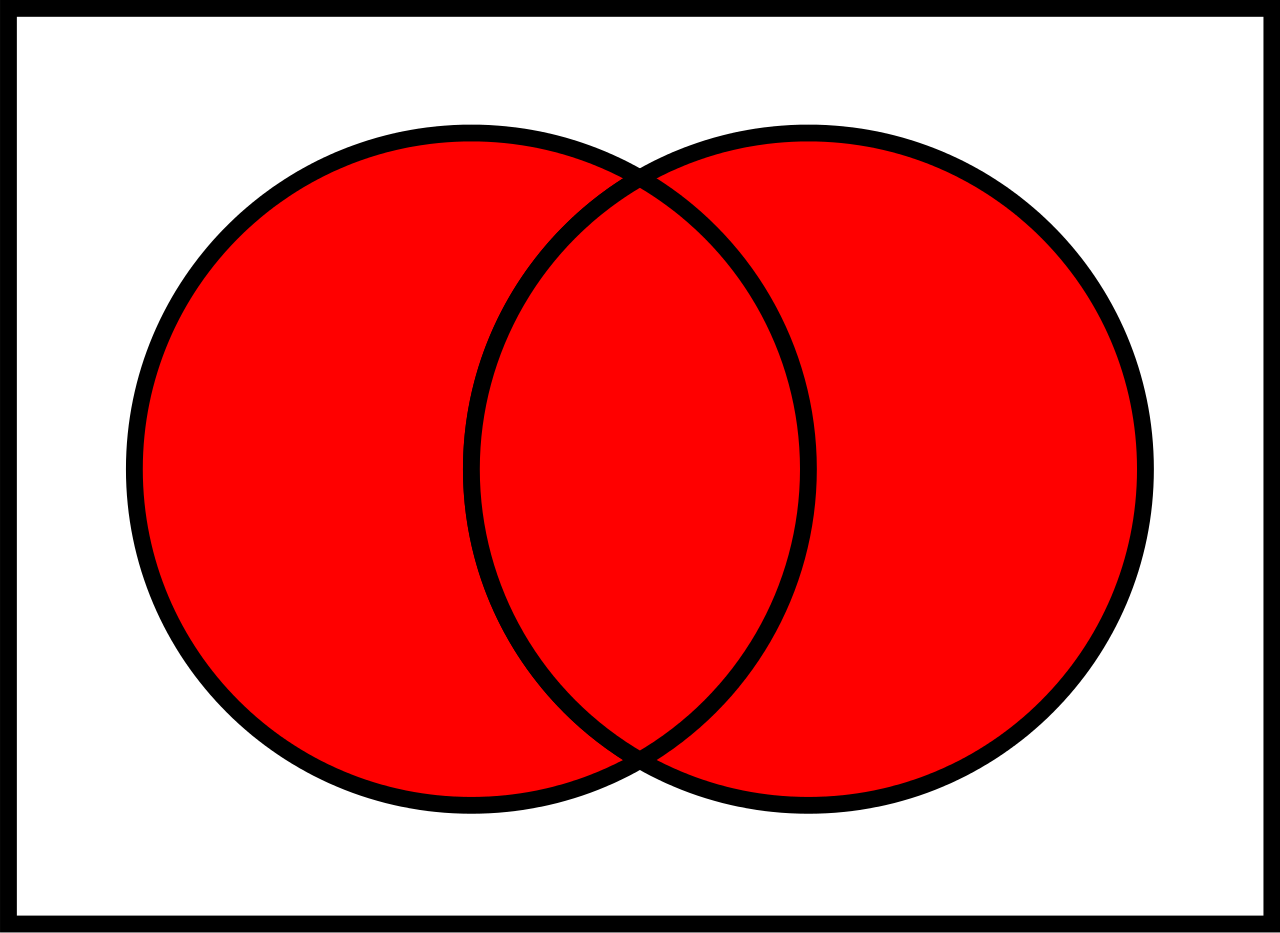
\includegraphics[width=2.5cm]{images/union.png} }}%
        \qquad
        \subfloat[\centering $A \cap B$]{{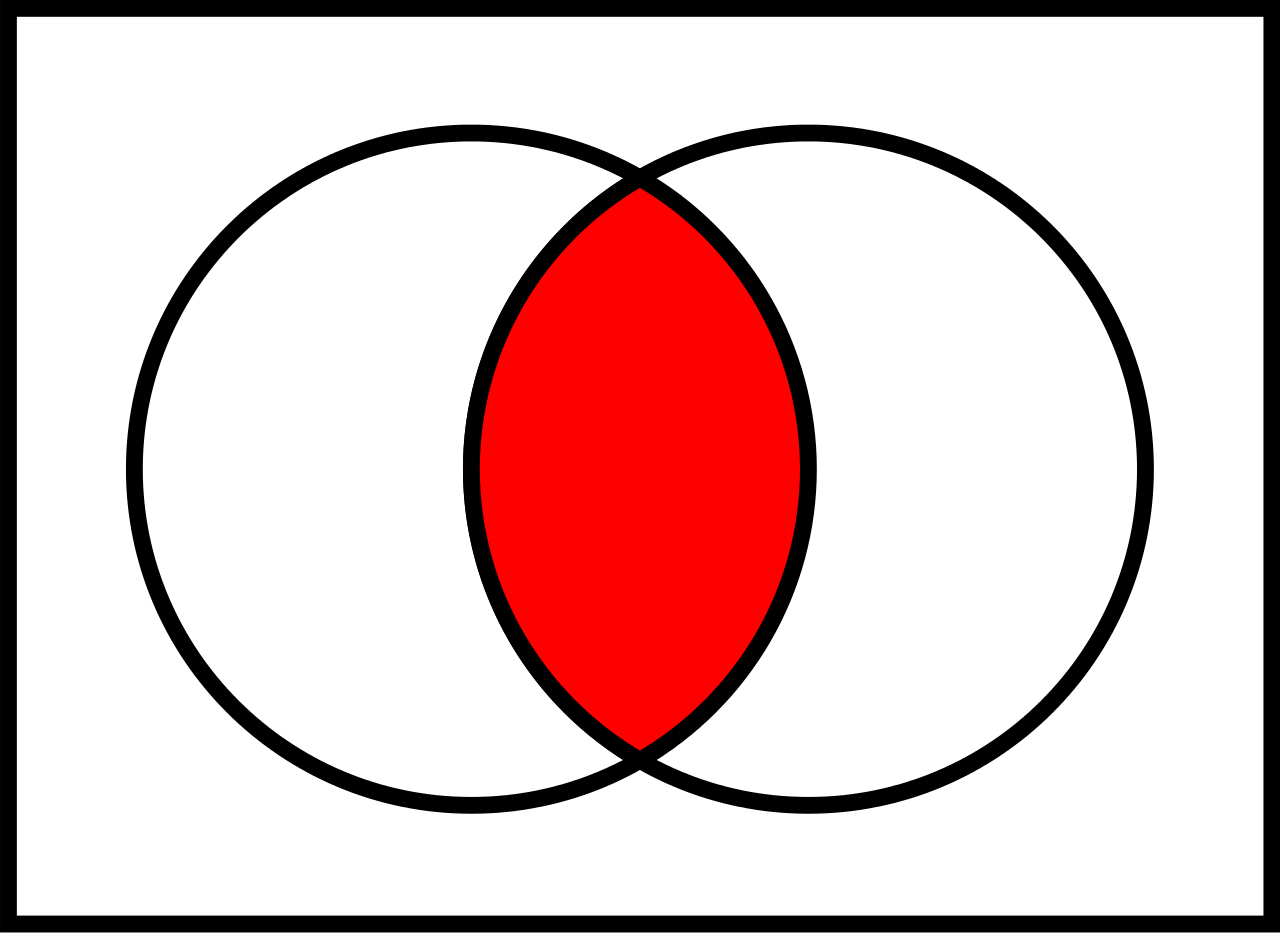
\includegraphics[width=2.5cm]{images/snitt.png} }}%
        \qquad
        \subfloat[\centering $B - A$]{{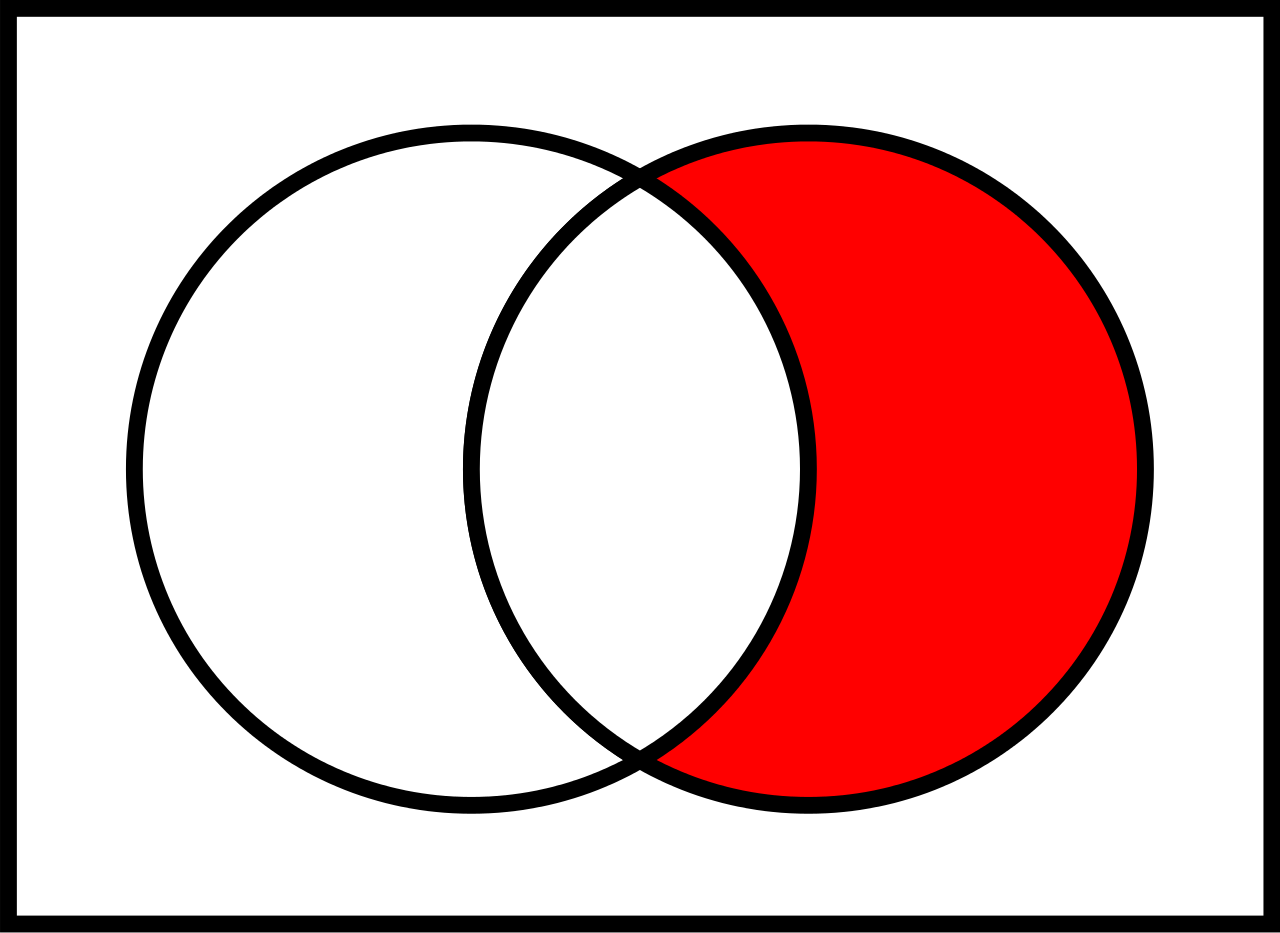
\includegraphics[width=2.5cm]{images/minus.png} }}%
        \qquad
        \subfloat[\centering $\bar{A}$]{{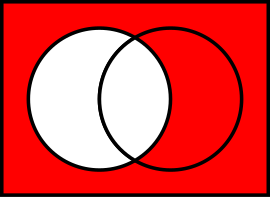
\includegraphics[width=2.5cm]{images/complement.png} }}%
        % \caption{Vennediagramer}%
        \label{fig:example2}%
    \end{figure}
\end{frame}

\begin{frame}{$\subset, \subseteq, =, \supseteq, \supset$}
    Vi har flere måter å uttrykke at et sett inneholder elementer fra et annet sett.
    \begin{itemize}
        \item $A \subseteq B := \forall x \in A : (x \in B)$
        %\item $A \supseteq B := B \subseteq A$
        \item $A \subset B := A \subseteq B \land \exists x \in B : (x \notin A)$
        %\item $A \supset B := B \subset A$
        \item $A = B := A \subseteq B \land B \subseteq A$
    \end{itemize}
    \pause
    \begin{block}{Eksempler}
        $\{1\} \subseteq \{1, 2\}$ = T\\
        $\{1\} \subseteq \{5\}$ = F\\
        $\{a, b\} \subset \{a, b\}$ = F\\
        $\{a, b\} \subseteq \{a, b\}$ = T
    \end{block}
    \pause
    \centering
    Obs! Enkelte skriver $\subset$ når de mener $\subseteq$, og $\subsetneq$ når de mener $\subset$.
\end{frame}

\begin{frame}{Tavleoppgaver fra H19}
    \begin{itemize}
        \item Vis eller motbevis at $(A - C) \cap (B - C) = \emptyset.$
        \item Vis eller motbevis at $(A - C) \cap (C - B) = \emptyset.$
    \end{itemize}
    
    For å løse det med vennediagrammer:
    \begin{enumerate}
        \item Tegn et vennediagram. Begynn med sirkler for A, B, etc.
        \item Fargelegg områdene til deluttrykkene, dvs $(A - C)$ og $(B - C)$ i dette eksemplet.
        \item Bruk områdene i deluttrykkene til å farge omårdene i de større uttrykkene, dvs hele $(A - C) \cap (B - C)$ her.
        \item Er områdene til hele uttrykkene på hver side av = det samme?
    \end{enumerate}
    \pause
    Alternativt: bruk definisjonene til $\cap$, $\cup$, etc til å omformulere uttrykket.
\end{frame}

\begin{frame}{Nyttige regler for sett}
        \begin{tabular}{l|c}
        Ekvivalens & Navn \\ \hline
        $A \cap U = A$ & Identity\\
        $A \cup \emptyset = A$ \\ \hline
        
        $A \cup U = U$ & Domination\\
        $A \cap \emptyset = \emptyset$\\ \hline
        
        $A \cup A = A$ & Idempotent\\
        $A \cap A = A$ \\ \hline
        
        $A = (A^C)^C$ & Negation\\ \hline
        
        $A \cup B = B \cup A$ & Commutative\\
        $A \cap B = B \cap A$ \\

    \end{tabular}
    \hfill
        \begin{tabular}{l|c}
        Ekvivalens & Navn \\ \hline
        
        $(A \cup B) \cup C = A \cup (B \cup C)$ & Associative\\
        $(A \cap B) \cap C = A \cap (B \cap C)$ \\ \hline
        
        $A \cup (B \cap C) = (A \cup B) \cap (A \cup C)$ & Distributive\\
        $A \cap (B \cup C) = (A \cap B) \cup (A \cap C)$ \\ \hline
        
        $(A \cap B)^C = A^C \cup B^C$ & De Morgan \\
        $(A \cup B)^C = A^C \cap B^C$ \\ \hline
        
        $A \cup (A \cap B) = A$ & Absorption \\
        $A \cap (A \cup B) = A$ \\ \hline
        
        $A \cup A^C = U$ & Negation \\
        $A \cap A^C = \emptyset$ \\
        \end{tabular}
\end{frame}

\begin{frame}{Kardinalitet}
    Om $A$ er et sett, er $\|A\|$ antall elementer i settet, \textit{kardinaliteten}, eller \textit{lengden}.\\
    To sett har samme kardinalitet om de har samme lengde.
    \begin{block}{Eksempler}
        $|\{a, b, c\}| = 3$ \\
        $|\{\}| = |\emptyset| = 0$\\
        $|\mathbb{N}| = \aleph_0$
    \end{block}
\end{frame}

\subsection{Funksjoner}
\begin{frame}{Funksjoner}
    Funksjoner kjenner vi fra INF100 i fjor. Nå skal vi formalisere dem litt mer.\\
    \begin{columns}
        \begin{column}{0.5\textwidth}
            Fra nå av ser vi på datatyper som sett:
            \begin{itemize}
                \item $int := \mathbb{Z}$
                \item $str := \{$ "a", "b", "c", "aa", "ab", ... $\}$
            \end{itemize}
            Domenet til en funksjon er inputsettet.\\
            Kodomenet til en funksjon er outputsettet.
        \end{column}
        \pause
        \begin{column}{0.5\textwidth}
            \begin{figure}
               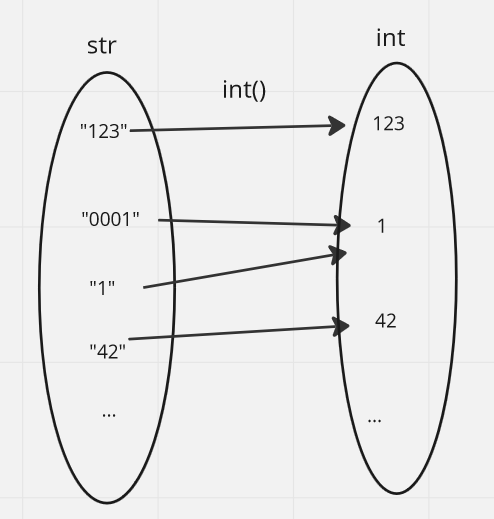
\includegraphics[scale = 0.4]{images/int.png} 
               \caption{$int : str \rightarrow int$}
            \end{figure}   
        \end{column}
    \end{columns}
\end{frame}

\begin{frame}{Funksjonskomposisjon}
    \begin{columns}
    \begin{column}{0.38\textwidth}
Gitt to funksjoner:
    \begin{itemize}
        \item $f : A \rightarrow B$
        \item $g : B \rightarrow C$
    \end{itemize}
Kan vi definere en unik tredje funksjon: \\
    $g \circ f : A \rightarrow C$\\
    $g \circ f := g(f(x))$\\
    \pause
    \end{column}
    \begin{column}{0.55\textwidth}
        \centering
        La $f(x) := x+1$, og $g(x) := x/2$.\\
        Da er $g \circ f = g(f(x)) = (x+1)/2$.\\
        \begin{figure}
            \centering
            \subfloat{{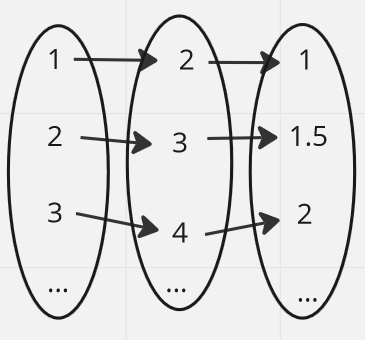
\includegraphics[width=2.8cm]{images/f, g.png} }}%
            \qquad
            \subfloat{{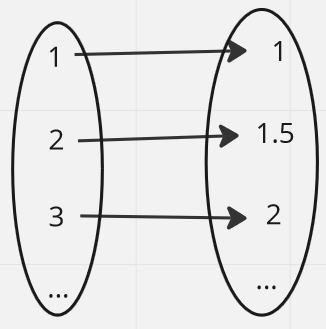
\includegraphics[width=2.8cm]{images/g o f.png} }}%
            \label{fig:g o f}
        \end{figure}
    \end{column}
    \end{columns}
    \pause
    Obs! Rekkefølgen er uintuitiv. $f$ skjer før $g$. Dere kan lese det som $g$ 'anvendt på' $f$.
\end{frame}

\begin{frame}{Injektivitet}
En funksjon $f : A \rightarrow B$ er \emph{injektiv} hvis $\forall a_1, a_2 \in A : [f(a_1) = f(a_2) \rightarrow a_1 = a_2]$.\\
Med andre ord: alle inputs gir et unikt output og alle piler peker på forskjellige ting.
    \begin{figure}%
        \centering
        \subfloat[\centering Ikke injektiv]{{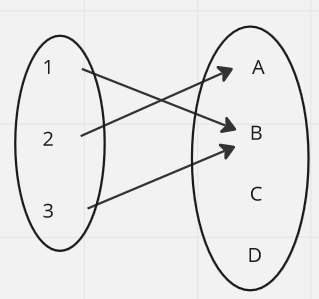
\includegraphics[width=3.2cm]{images/Ikke inj.png} }}%
        \qquad
        \subfloat[\centering Injektiv]{{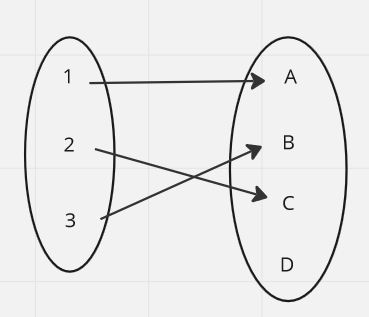
\includegraphics[width=3.2cm]{images/Inj.png} }}%
        \qquad
        \subfloat[\centering Ikke injektiv]{{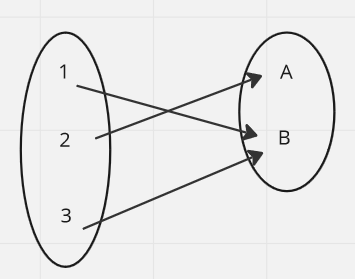
\includegraphics[width=3.2cm]{images/Heller ikke inj.png} }}%
        \label{fig:inj}%
    \end{figure}
    \pause
    Observer at det finnes en injeksjon hvos og bare hvis $|B| \geq |A|$.
\end{frame}

\begin{frame}{Surjektivitet}
En funksjon $f : A \rightarrow B$ er \emph{surjektiv} hvis $\forall b \in B$ $\exists a \in A: [f(a) = b]$.\\
Med andre ord: hele kodomenet/outputsettet blir brukt og alt i $B$ har minst én pil som peker på seg.
    \begin{figure}%
        \centering
        \subfloat[\centering Ikke surjektiv]{{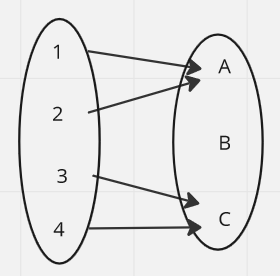
\includegraphics[width=3.2cm]{images/Ikke surjektiv.png} }}%
        \qquad
        \subfloat[\centering Surjektiv]{{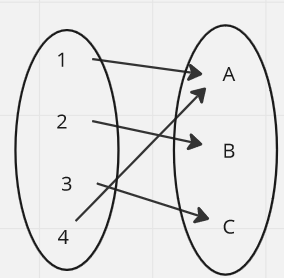
\includegraphics[width=3.2cm]{images/Surjektiv.png} }}%
        \qquad
        \subfloat[\centering Ikke surjektiv]{{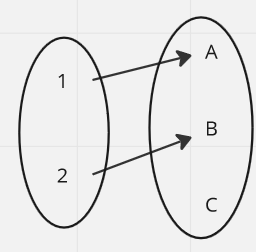
\includegraphics[width=3.2cm]{images/Aldri surjektiv.png} }}%
        \label{fig:sur}
    \end{figure}
    \pause
    Observer at det finnes en surjeksjon hvis og bare hvis $|A| \geq |B|$.
\end{frame}

\begin{frame}{Bijektivitet}
En funksjon $f : A \rightarrow B$ er \emph{Bijektiv} om den er både injektiv og surjektiv.\\
    \pause
    Da finnes det en unik invers funksjon $f^{-1} : B \rightarrow A$ slik at $f^{-1} \circ f = id_A$ og $f \circ f^{-1} = id_B$, dvs at $\forall a \in A : [a = f^{-1}(f(a))]$ og $\forall b \in B : [b = f(f^{-1}(b))]$.
    \pause
\begin{figure}
        \centering
        \subfloat[\centering Surjektiv, ikke injektiv]{{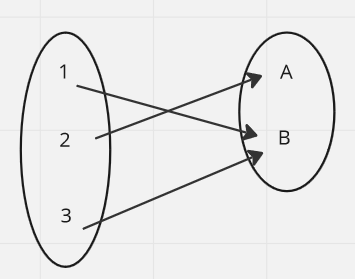
\includegraphics[width=2.4cm]{images/Heller ikke inj.png} }}%
        \qquad
        \subfloat[\centering Injektiv, ikke surjektiv]{{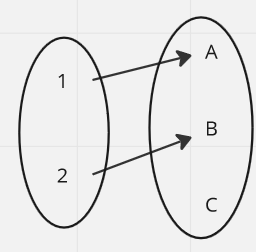
\includegraphics[width=2.4cm]{images/Aldri surjektiv.png} }}%
        \qquad
        \subfloat[\centering Bijektiv]{{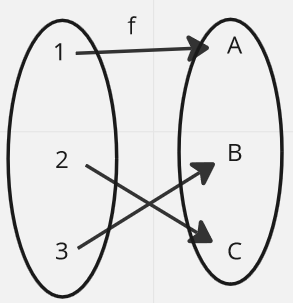
\includegraphics[width=2.4cm]{images/Bijektiv f.png} }}
        \qquad
        \subfloat[\centering Inverset $f^{-1}$]{{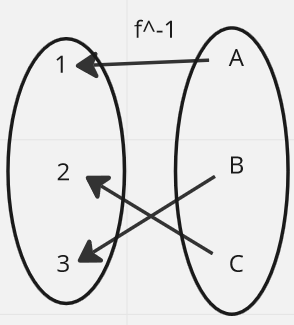
\includegraphics[width=2.4cm]{images/Invers f.png} }}%
        \label{fig:bij}
    \end{figure}

    \pause
    Observer at det finnes en bijeksjon hvis og bare hvis $|A| = |B|$.
\end{frame}

\begin{frame}{Tavleoppgaver om injektivitet, surjektivitet, bijektivitet}
    \begin{itemize}
        \item Injektiv:  $\forall a_1, a_2 : [f(a_1) = f(a_2) \rightarrow a_1 = a_2]$.\\
        \item Surjektiv: $\forall b \in B$  $\exists a \in A : [f(a) = b]$.\\
        \item Bijektiv: begge de over \\
    \end{itemize}
    \pause
    \begin{block}{Avgjør om de følgende funksjonene er injektive, surjektive, eller bijektive:}
        $even : \mathbb{Z} \rightarrow $ Bool, $even(x) := x$ mod $2 = 0$\\
        $f : \mathbb{R} \rightarrow \mathbb{R}$, $g(x) := e^x$\\
        $g : \mathbb{R} \rightarrow \mathbb{R}^+$, $g(x) := e^x$\\
        $h : \mathbb{R} \rightarrow \mathbb{R}$, $h(x) := 2x + 1$\\
        $k : \mathbb{Q} \rightarrow \mathbb{N}$, $k(x) := 1$\\
    \end{block}
    \pause
    Noen kaller surjektive funksjoner for 'onto' på engelsk. Mens 'one-to-one', eller 1-1, kan bety enten bijektiv og injektiv avhengig av hvem som sier det.
\end{frame}

\subsection{Tellbarhet}
\begin{frame}{Hva er størst av $|\mathbb{N}|$ og $|\mathbb{Z}|$?}
    \begin{columns}
    \begin{column}{0.35\textwidth}
        $\mathbb{N} = \{0, 1, 2, 3, 4, ...\}$\\
        $\mathbb{Z} = \{..., -2, -1, 0, 1, 2, ...\}$\\[5mm]
        \pause
        Vi definerer en bijeksjon:\\ 
        $f : \mathbb{N} \rightarrow \mathbb{Z}$
        $f(n) :=
        \begin{cases}
            \frac{n}{2}, n \text{ mod } 2 = 0\\
            -\frac{n+1}{2}, \text{otherwise}\\
        \end{cases}$\\[5mm]
        Konklusjon: $|\mathbb{N}|$ = $|\mathbb{Z}|$ = $\aleph_0$. 
    \end{column}
    \begin{column}{0.6\textwidth}
        \begin{figure}
            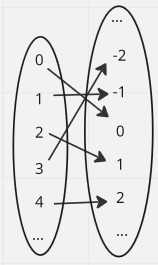
\includegraphics[scale=0.75]{images/n eq eq z.png}
        \end{figure}
    \end{column}
    \end{columns}    
\end{frame}

\begin{frame}{Hva er størst av $|\mathbb{N}|$ og $|\mathbb{Q}|$?}
        $\mathbb{N} = \{0, 1, 2, 3, 4, ...\}$\\
        $\mathbb{Q} = \{a / b | a\in \mathbb{Z}, b \in \mathbb{Z}\}$\\[2mm]
        \pause
        Vi definerer en bijeksjon $g : \mathbb{N} \rightarrow \mathbb{Q}$:\\
        $f(0) := 1$\\
        $f(n) := \frac{1}{2\lfloor f(n-1) \rfloor - f(n-1)+1}$\\
        $g(0) := 0$\\
        $g(2n) := f(n)$\\
        $g(2n-1) := -f(n)$\\
        Konklusjon: $|\mathbb{N}|$ = $|\mathbb{Q}|$ = $\aleph_0$.\\[2mm]\pause
        Derimot er $|\mathbb{R}| > |\mathbb{N}|$, og vi skriver at $|\mathbb{R}| = \aleph_1$.\\ 
        For en enkel forklaring med et eksempel, se Veritasiums video om Hilberts Hotell: \url{https://www.youtube.com/watch?v=OxGsU8oIWjY}
\end{frame}

\subsection*{Spørretid}
\begin{frame}{Spørsmål?}
    \begin{figure}
        \centering
        
\includegraphics[height = 4.9cm]{images/guillaume4.jpg}
        \caption{Guillaume på Vidden}
        \label{fig:guillaume4}
    \end{figure}
\end{frame}